\graphicspath{{Figures/}}

\title{\fontsize{33}{45}{\huge Pattern Classification (EET 3035)\newline \vspace{8pt} \Large Extra Lecture: 2D-Gabor Filters\vspace{-1.1cm}}}
\author{\vspace{-0.4cm}\\\normalsize{\bf Dr. Kundan Kumar}\\ PhD (IIT Kharagpur)\\
Associate Professor\\Department of ECE}
% - Give the names in the same order as the appear in the paper.
% - Use the \inst{?} command only if the authors have different
%   affiliation.

\institute[Indian Institute of Technology Kharagpur] % (optional, but mostly needed)
{

\includegraphics[height=.17\textheight]{SOAlogo.png}\\
 Faculty of Engineering (ITER)\\ S`O'A Deemed to be University, Bhubaneswar, India-751030\\
 \copyright\  2020 Kundan Kumar, All Rights Reserved\\
  \vspace{-1.1cm}}
% - Use the \inst command only if there are several affiliations.
% - Keep it simple, no one is interested in your street address.
\date{}
% To remove page number from a perticular slide
{
\setbeamertemplate{logo}{}
\makeatletter
\setbeamertemplate{footline}{
        \leavevmode%
  
  % First line.
  \hbox{%
  \begin{beamercolorbox}[wd=.2\paperwidth,ht=\beamer@decolines@lineup,dp=0pt]{}%
  \end{beamercolorbox}%
  \begin{beamercolorbox}[wd=.8\paperwidth,ht=\beamer@decolines@lineup,dp=0pt]{lineup}%
  \end{beamercolorbox}%
  } %
  % Second line.
  \hbox{%
  \begin{beamercolorbox}[wd=\paperwidth,ht=\beamer@decolines@linemid,dp=0pt]{linemid}%
  \end{beamercolorbox}%
  } %
  % Third line.
  \hbox{%
  \begin{beamercolorbox}[wd=.1\paperwidth,ht=\beamer@decolines@linebottom,dp=0pt]{}%
  \end{beamercolorbox}%
  \begin{beamercolorbox}[wd=.9\paperwidth,ht=\beamer@decolines@linebottom,dp=0pt]{linebottom}%
  \end{beamercolorbox}%
  }%
        }
\makeatother
\begin{frame}
\titlepage
\end{frame}
}


\begin{frame}[label=4]{Outline}
\tableofcontents
\note{}
\end{frame}

\section{Introduction}
\subsection{}
\begin{frame}{Introduction}
\begin{itemize}
\item Gabor filters are bandpass filters which are used in image processing for
\begin{itemize}
\item feature extraction,
\item texture analysis,
\item stereo disparity estimation, etc.
\end{itemize}   
\item The kernel  mask of these filters is created by multiplying a Gaussian envelop function with a complex oscillation.
\begin{equation}
{g_{\lambda ,\theta ,\varphi ,\sigma ,\gamma }}(x,y) = \exp \left( { - \frac{{x{'^2} + {\gamma ^2}y{'^2}}}{{2{\sigma ^2}}}} \right)\exp \left( i\left({2\pi \frac{{x'}}{\lambda } + \varphi }\right) \right)\nonumber
\end{equation}
\item It was shown by several researchers that the profile of simple-cell receptive fields in the mammalian visual cortex can by described by oriented two-dimensional Gabor functions.
\end{itemize}
\end{frame}

\begin{frame}{Visual Cortex}
\begin{figure}
\includegraphics[scale=0.28,angle =90]{visualCortex.png}
\caption{Broadmann area 17~\footfullcite{wikiVisualCortex}}
\end{figure}
\end{frame}

\begin{frame}{Visual System}
\begin{itemize}
\item In the spatial domain, a 2D Gabor filter is a Gaussian kernel function modulated by a sinusoidal plane wave. 
\item Some authors claim that simple cells in the visual cortex of mammalian brains can be modelled by Gabor functions.
\item Simple cells respond to bars and gratings of given
orientation.
\begin{figure}
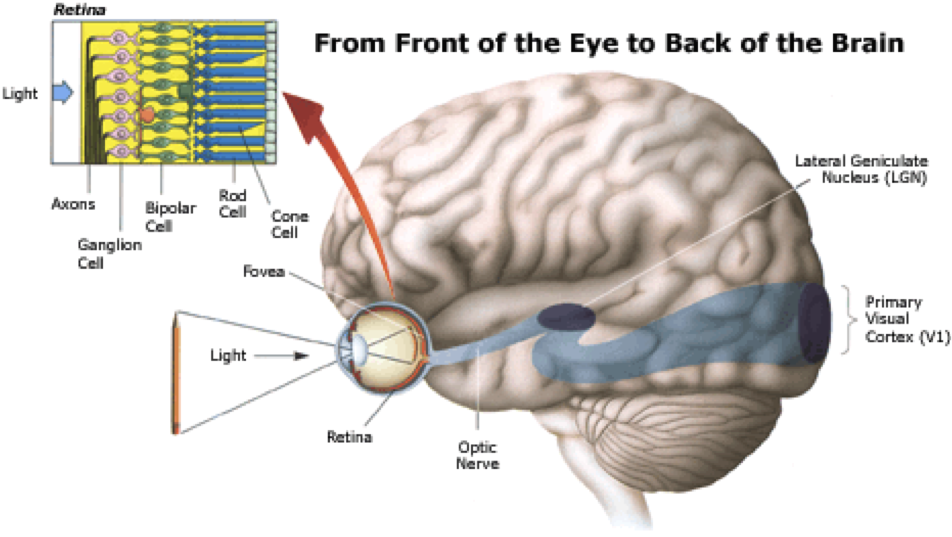
\includegraphics[scale=0.52]{visualSystem.png}
\end{figure}
\end{itemize}
\end{frame}

\begin{frame}{2D Gabor Functions}
\begin{itemize}
\item Complex
\begin{equation}
{g_{\lambda ,\theta ,\varphi ,\sigma ,\gamma }}(x,y) = \exp \left( { - \frac{{x{'^2} + {\gamma ^2}y{'^2}}}{{2{\sigma ^2}}}} \right)\exp \left( i\left({2\pi \frac{{x'}}{\lambda } + \varphi }\right) \right)\nonumber
\end{equation}
\item Real
\begin{equation}
{g_{\lambda ,\theta ,\varphi ,\sigma ,\gamma }}(x,y) = \exp \left( { - \frac{{x{'^2} + {\gamma ^2}y{'^2}}}{{2{\sigma ^2}}}} \right)\cos \left( {2\pi \frac{{x'}}{\lambda } + \varphi } \right)\nonumber
\end{equation}
\item Imaginary
\begin{equation}
{g_{\lambda ,\theta ,\varphi ,\sigma ,\gamma }}(x,y) = \exp \left( { - \frac{{x{'^2} + {\gamma ^2}y{'^2}}}{{2{\sigma ^2}}}} \right)\sin \left( {2\pi \frac{{x'}}{\lambda } + \varphi } \right)\nonumber
\end{equation}
where
\begin{align*}
x'=&x\cos \theta +y\sin \theta\\
y'=&-x\sin \theta +y\cos \theta\\
\end{align*}
\end{itemize}
\end{frame}
\section{Filter Parameter}
\subsection{}
\begin{frame}{2D Gabor function parameters}
\begin{equation}
{g_{\lambda ,\theta ,\varphi ,\sigma ,\gamma }}(x,y) = \exp \left( { - \frac{{x{'^2} + {\gamma ^2}y{'^2}}}{{2{\sigma ^2}}}} \right)\cos \left( {2\pi \frac{{x'}}{\lambda } + \varphi } \right)\nonumber
\end{equation}
where
\begin{align*}
x'=&x\cos \theta +y\sin \theta\\
y'=&-x\sin \theta +y\cos \theta\\
\end{align*}
$\lambda\rightarrow$ wavelength of the sinusoidal factor,\\
$\theta\rightarrow$ orientation of the normal to the parallel stripes of a Gabor function,\\
$\varphi\rightarrow$ phase offset,\\
$\sigma\rightarrow$ standard deviation of the Gaussian envelope,\\
$\gamma\rightarrow$ spatial aspect ratio, specifies the ellipticity of the support of the Gabor function.
\end{frame}

\begin{frame}{Wavelength ($\lambda$)}
\begin{itemize}
\item Wavelength of the cosine factor of the Gabor filter kernel.
\item Value is to be specified in number of pixels.
\item Valid values are real numbers, $\lambda\geq 2$
\item The value $\lambda=2$ should not be used in combination with phase offset $\phi = -90$ or $\phi=90$, because in these cases the Gabor function is sampled in its zero crossings.
\item To avoid undesirable effect at the image borders, $\lambda$ value should be smaller than one fifth of the input size.
\begin{figure}

\includegraphics[scale=0.8]{Gabor03}
\caption{Image size is $100\times 100$, $\lambda=5,10,15$ from left to right, other parameters $\theta = 0$, $\varphi = 0$, $\gamma=0.5$, $b = 1$}
\end{figure}
\end{itemize}
\end{frame}

\begin{frame}{Orientations ($\theta$)}
\begin{itemize}
\item This parameter specifies the orientation of the normal to the parallel stripes of a Gabor function.
\item Value is to be specified in degrees.
\item Valid values are real numbers between $0-360$.
\begin{figure}

\includegraphics[scale=1]{Gabor04}
\caption{Image size is $100\times 100$, $\theta=0,45,90$ from left to right, other parameters $\lambda = 10$, $\varphi= 0$, $\gamma=0.5$, $b = 1$}
\end{figure}
\end{itemize}
\end{frame}

\begin{frame}{Phase offset ($\varphi$)}
\begin{itemize}
\item The phase offset $\varphi$ in the cosine factor of the Gabor function is specified in degree.
\item Valid values are real number in between $-180$ and $180$.
\item The values 0 and 180 corresponds to center-symmetric `center-on' and `center-off' function, respectively. While $-90$ and $90$ corresponds to anti-symmetric functions
\begin{figure}

\includegraphics[scale=0.8]{Gabor06}
\caption{Image size is $100\times 100$, $\phi=0,~180,~-90,~and~90$ degrees from left to right, other parameters $\lambda = 10$, $\theta = 0$, $\gamma=0.5$, $b = 1$}
\end{figure}
\end{itemize}
\end{frame}

\begin{frame}{Aspect ratio ($\gamma$)}
\begin{itemize}
\item This is spatial aspect ratio which specifies the ellipticity of the support of the Gabor function.
\item For $\gamma=1$, the support is circular.
\item For $\gamma <1$ the support is elongated in orientation of the parallel stripes of the function
\item Normal value is $\gamma=0.5$
\begin{figure}

\includegraphics[scale=1]{Gabor07}
\caption{Image size is $100\times 100$, $\gamma=0.5~and~1$ degrees from left to right, other parameters $\lambda = 10$, $\theta = 0$, $\varphi=0$, $b = 1$}
\end{figure}
\end{itemize}
\end{frame}

\begin{frame}{Bandwidth ($b$)}
\begin{itemize}
\item The half-response spatial frequency bandwidth $b$ (in octaves)  of a Gabor filter is related to the ratio $\frac{\sigma}{\lambda}$.
%, where $\sigma$ and $\lambda$  are the standard deviation of the Gaussian factor of the Gabor function and the preferred wavelength, respectively.
\[b = {\log _2}\frac{{\frac{\sigma }{\lambda }\pi  + \sqrt {\frac{{\ln 2}}{2}} }}{{\frac{\sigma }{\lambda }\pi  - \sqrt {\frac{{\ln 2}}{2}} }},~~~\frac{\sigma }{\lambda } = \frac{1}{\pi }\sqrt {\frac{{\ln 2}}{2}}  \cdot \frac{{{2^b} + 1}}{{{2^b} - 1}}\]
\item The value of $\sigma$ cannot be specified directly. It can only be changed through the bandwidth $b$.
\item Must be a real positive number.
\item The smaller the bandwidth, the larger $\sigma$,
\end{itemize}
\end{frame}

\begin{frame}{Spatial frequency (${1}/{\lambda}$)}
\begin{itemize}
\item Preferred spatial frequency, ${1}/{\lambda}$, and size $\sigma$ are not fully independent. Values are related with a relation
\begin{equation}
\sigma = a\lambda \nonumber
\end{equation}
\item $a$ varies in between $0.03$ and $0.6$ for most cells.
\item In many experiments, $a=0.56$ is used, i.e., $\sigma=0.56\lambda$.
\begin{figure}
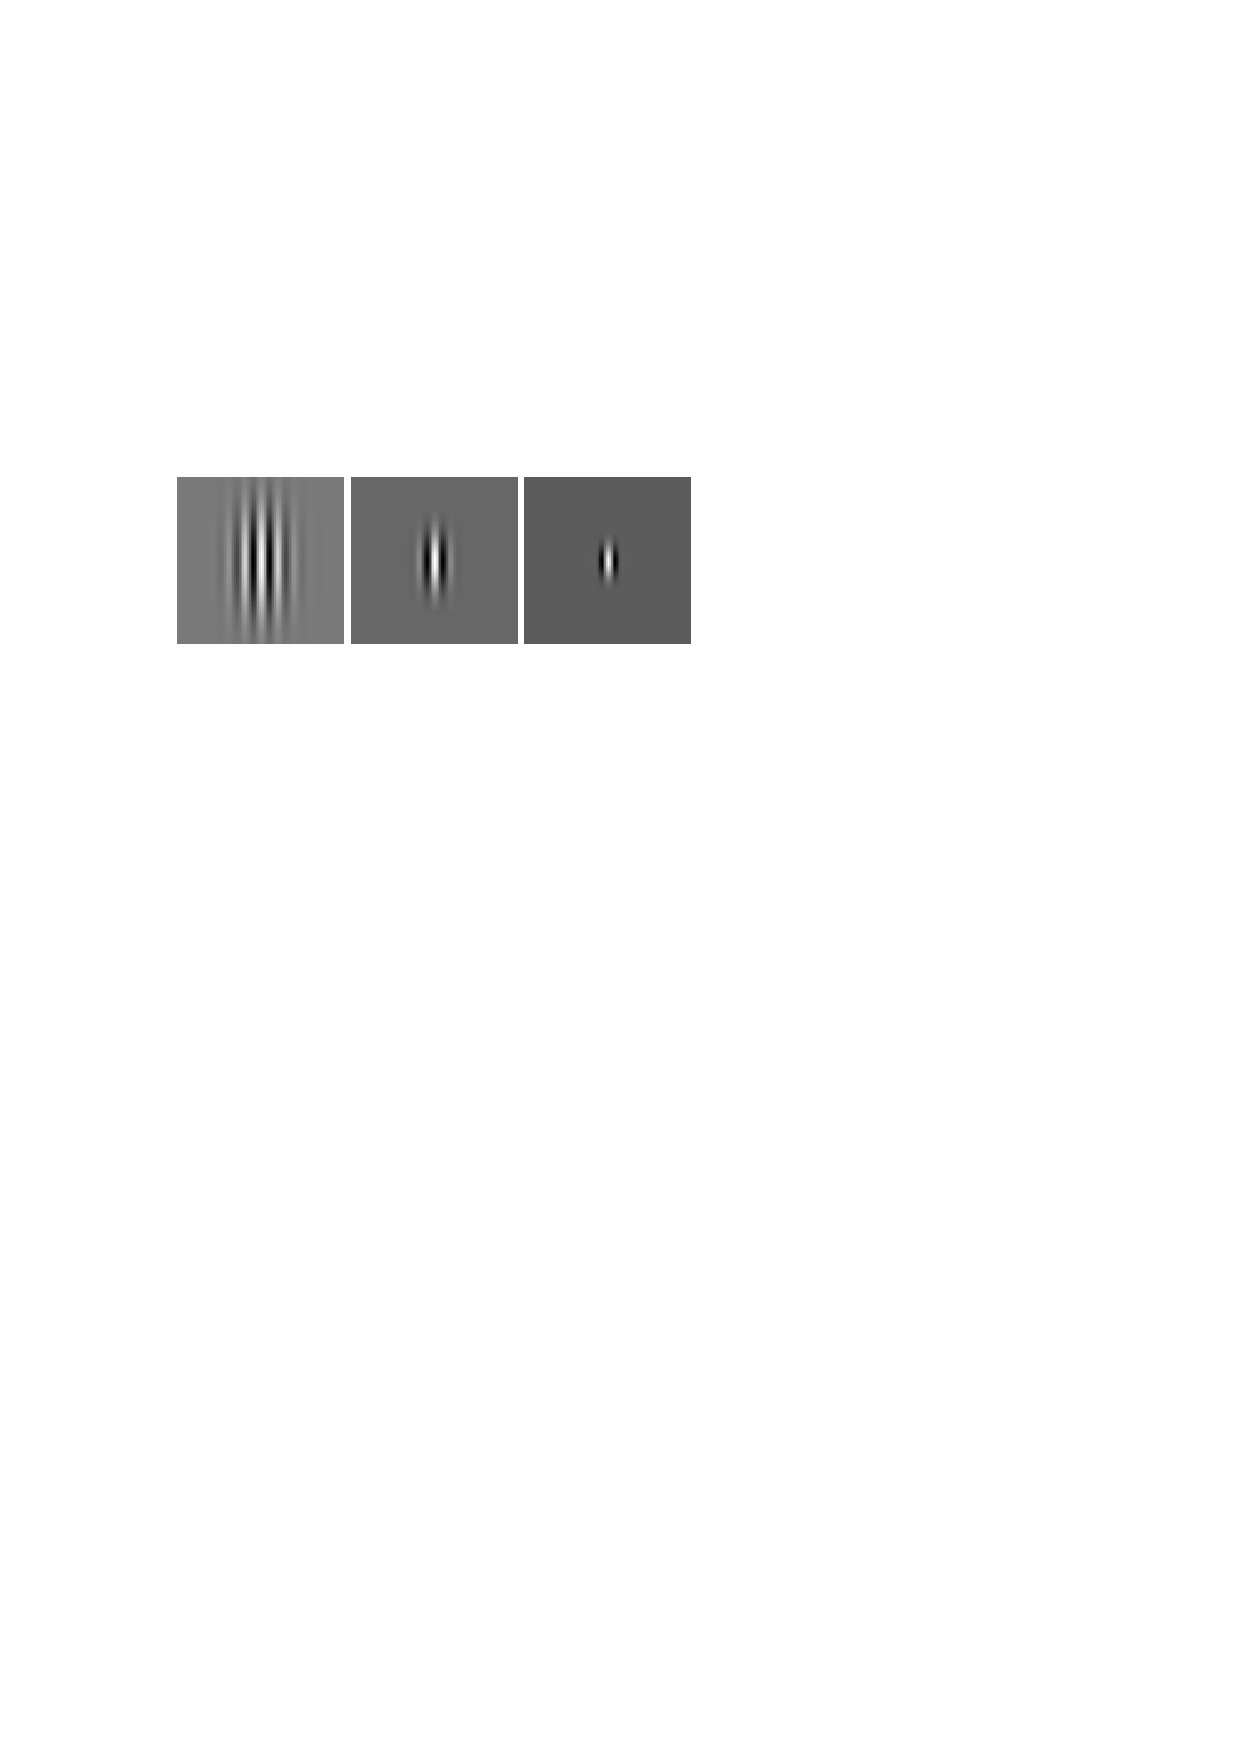
\includegraphics[scale=0.8]{Gabor08}
\caption{Image size is $100\times 100$, $b=0.5,~1$~and~$2$ from left to right, respectively. Other parameters $\lambda = 10$, $\theta = 0$, $\varphi=0$, $\gamma= 0.5$}.
\end{figure}
\end{itemize}
\end{frame}
\section{Applications}
\subsection{}
\begin{frame}{Set of Gabor filters}
\begin{figure}
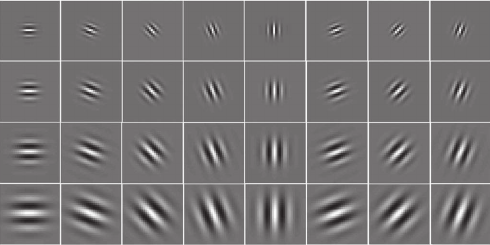
\includegraphics[scale=2.5]{Gabor14.png}
\end{figure}
\end{frame}

\begin{frame}{Application - Texture Segmentation}
\begin{figure}

\includegraphics[scale=0.9]{Gabor09}\\
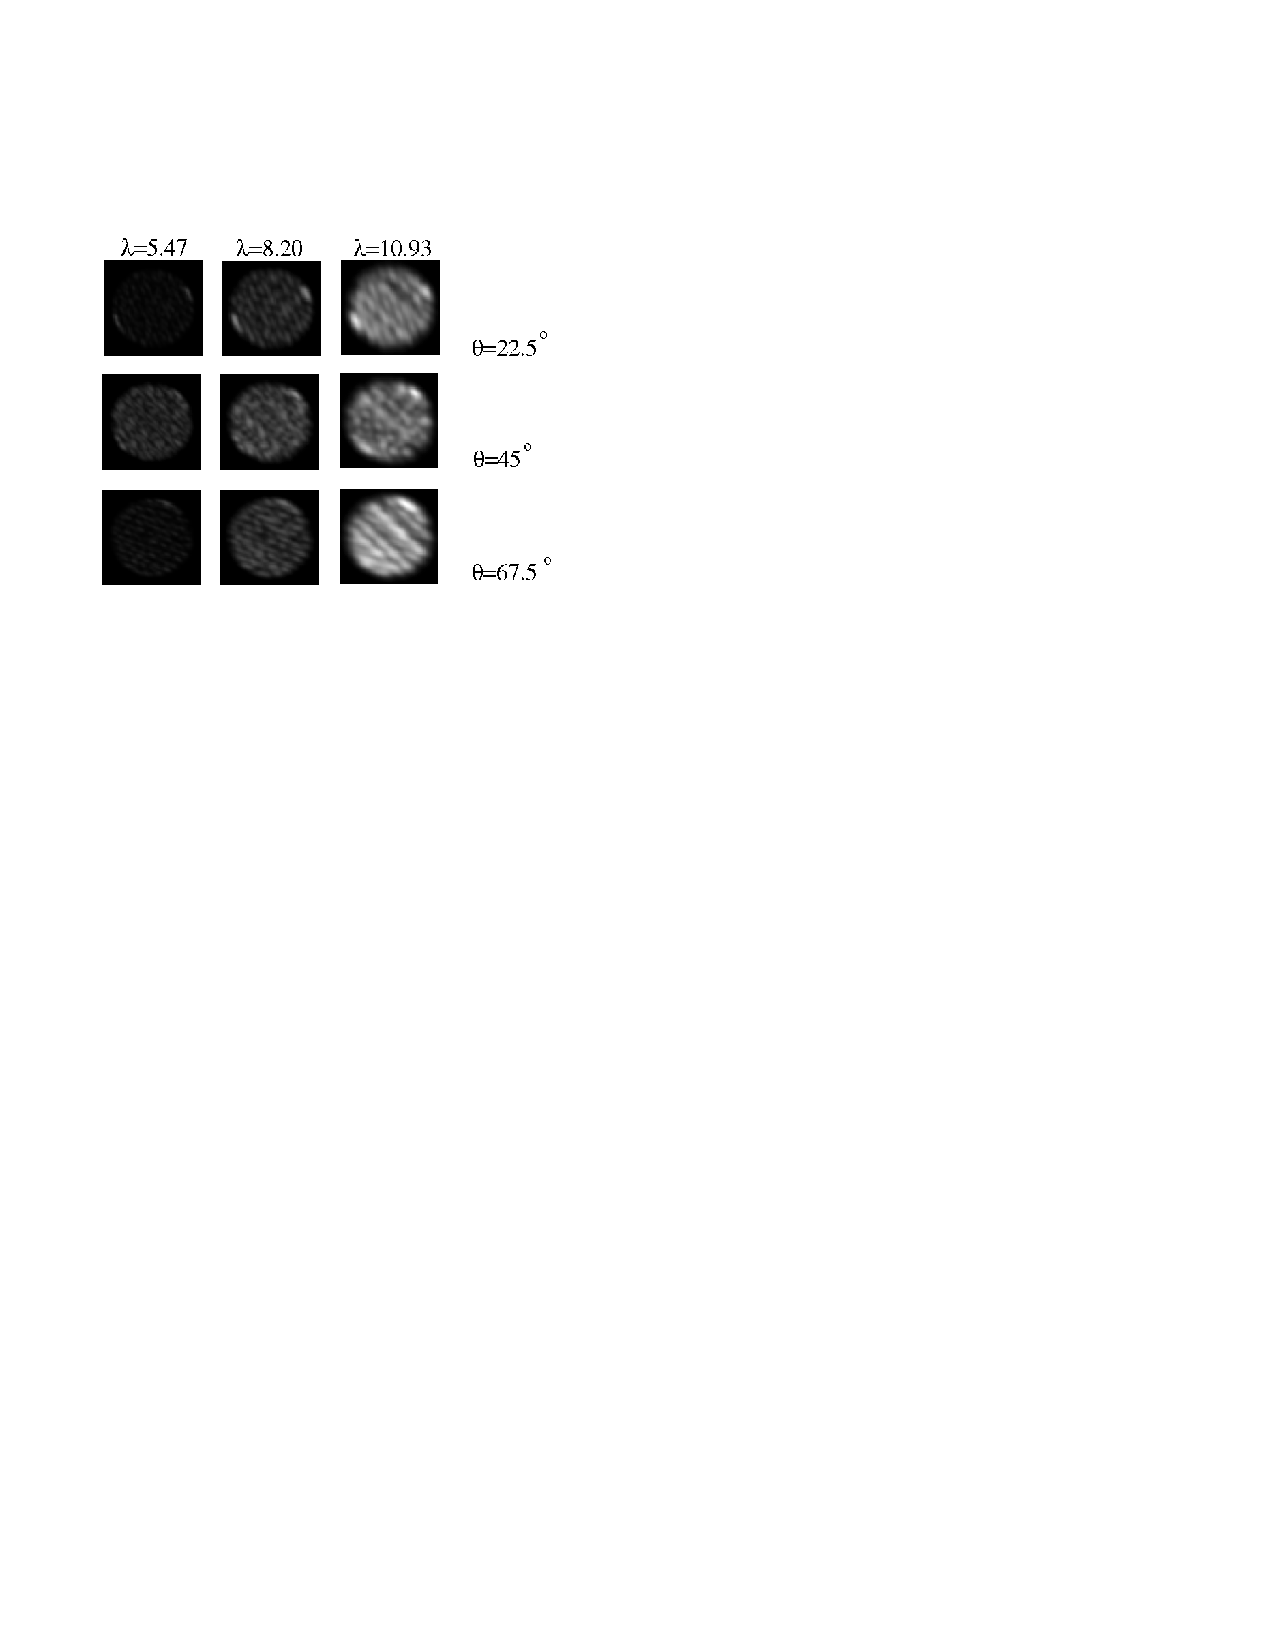
\includegraphics[scale=0.9]{Gabor10}
\end{figure}
\end{frame}

\begin{frame}{Application - Texture Segmentation}
\begin{figure}
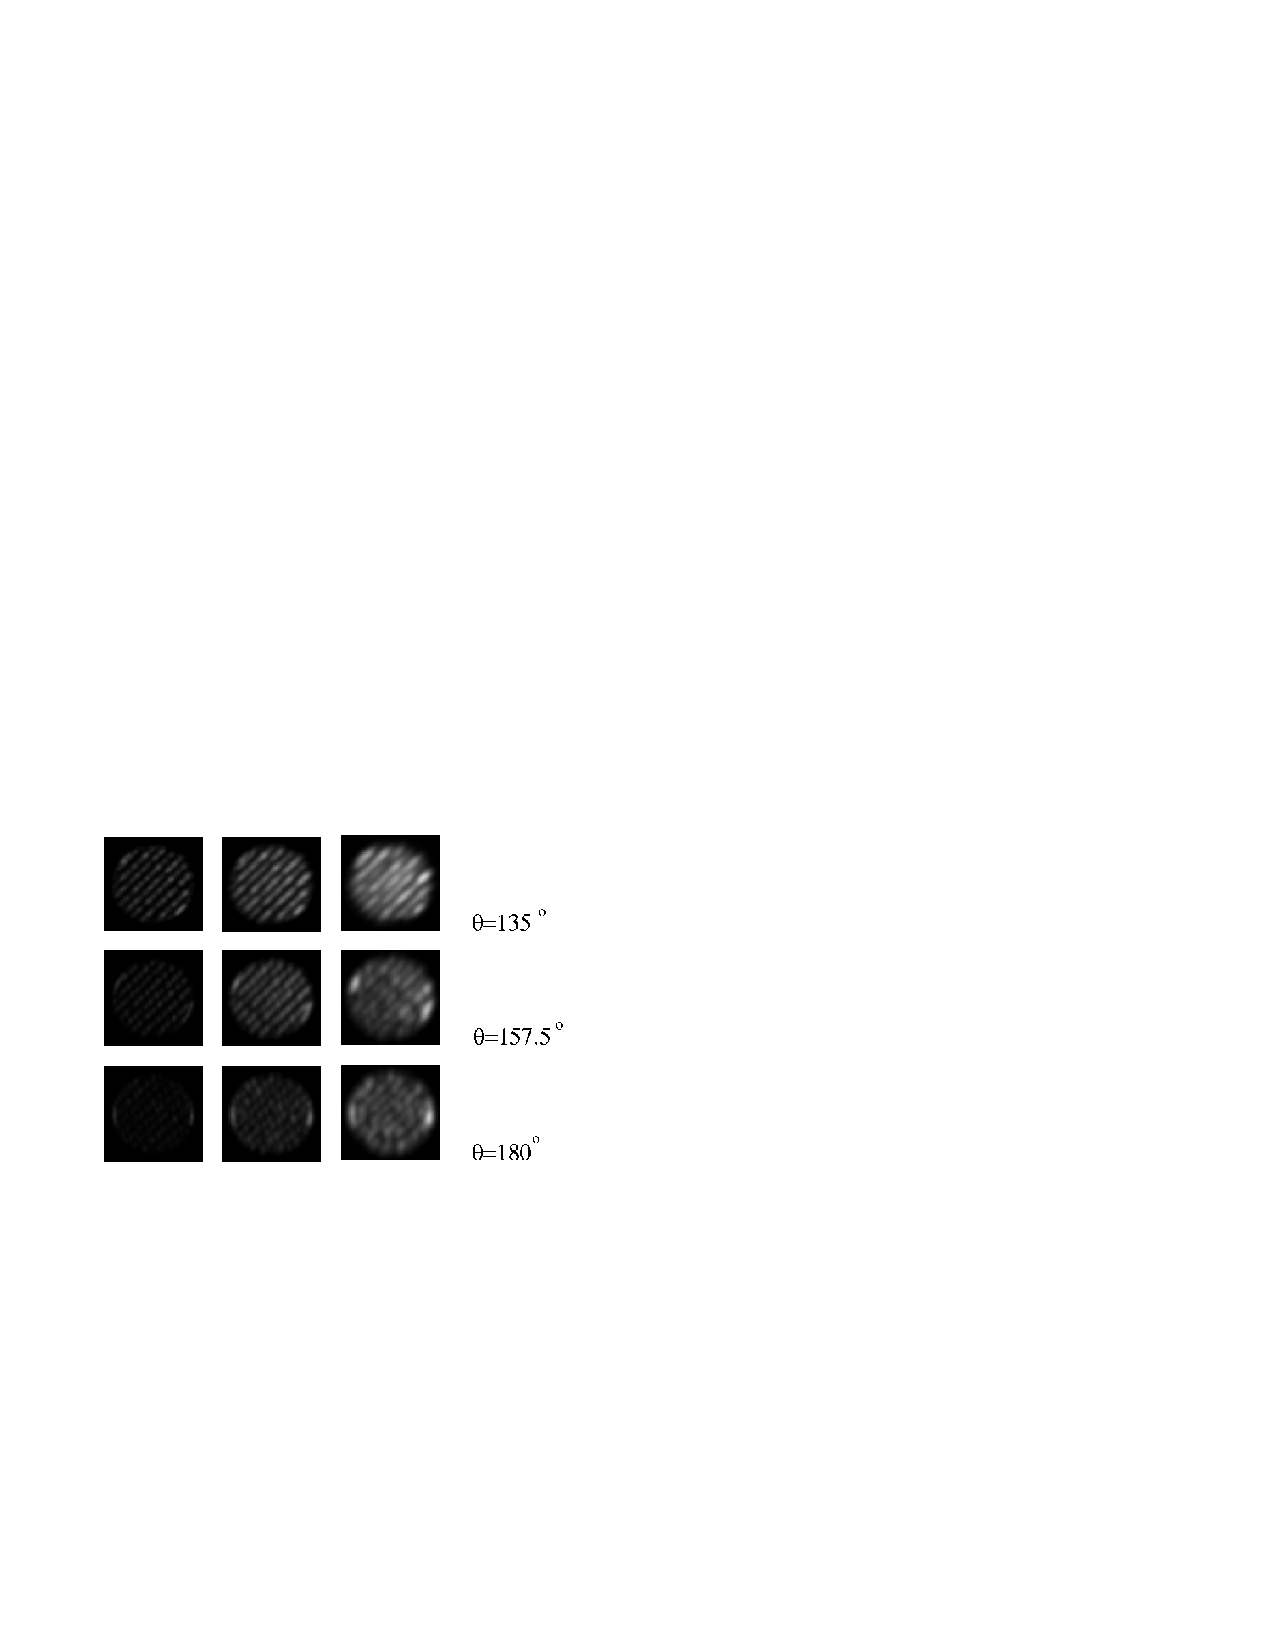
\includegraphics[scale=0.9]{Gabor11}\\
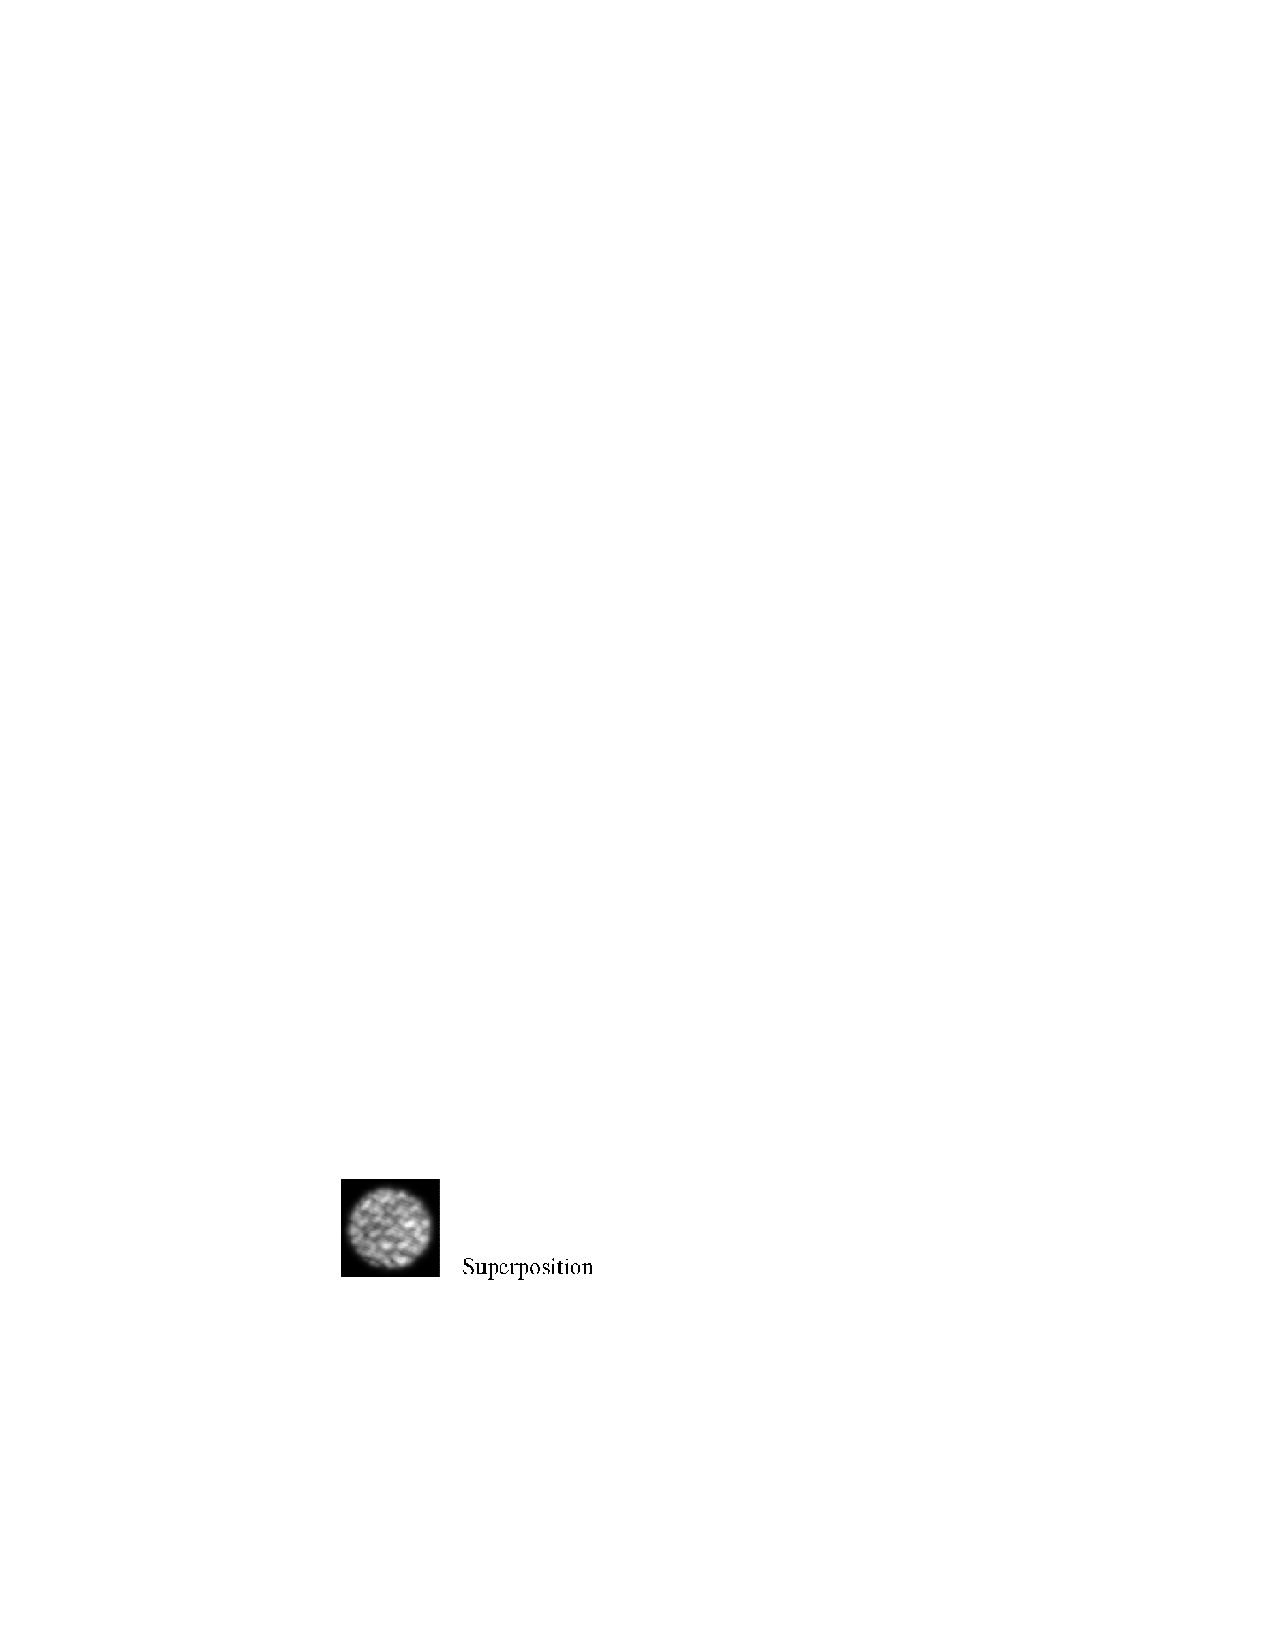
\includegraphics[scale=0.9]{Gabor12}
\end{figure}
\end{frame}

\begin{frame}{Application - Texture Segmentation}
\begin{figure}
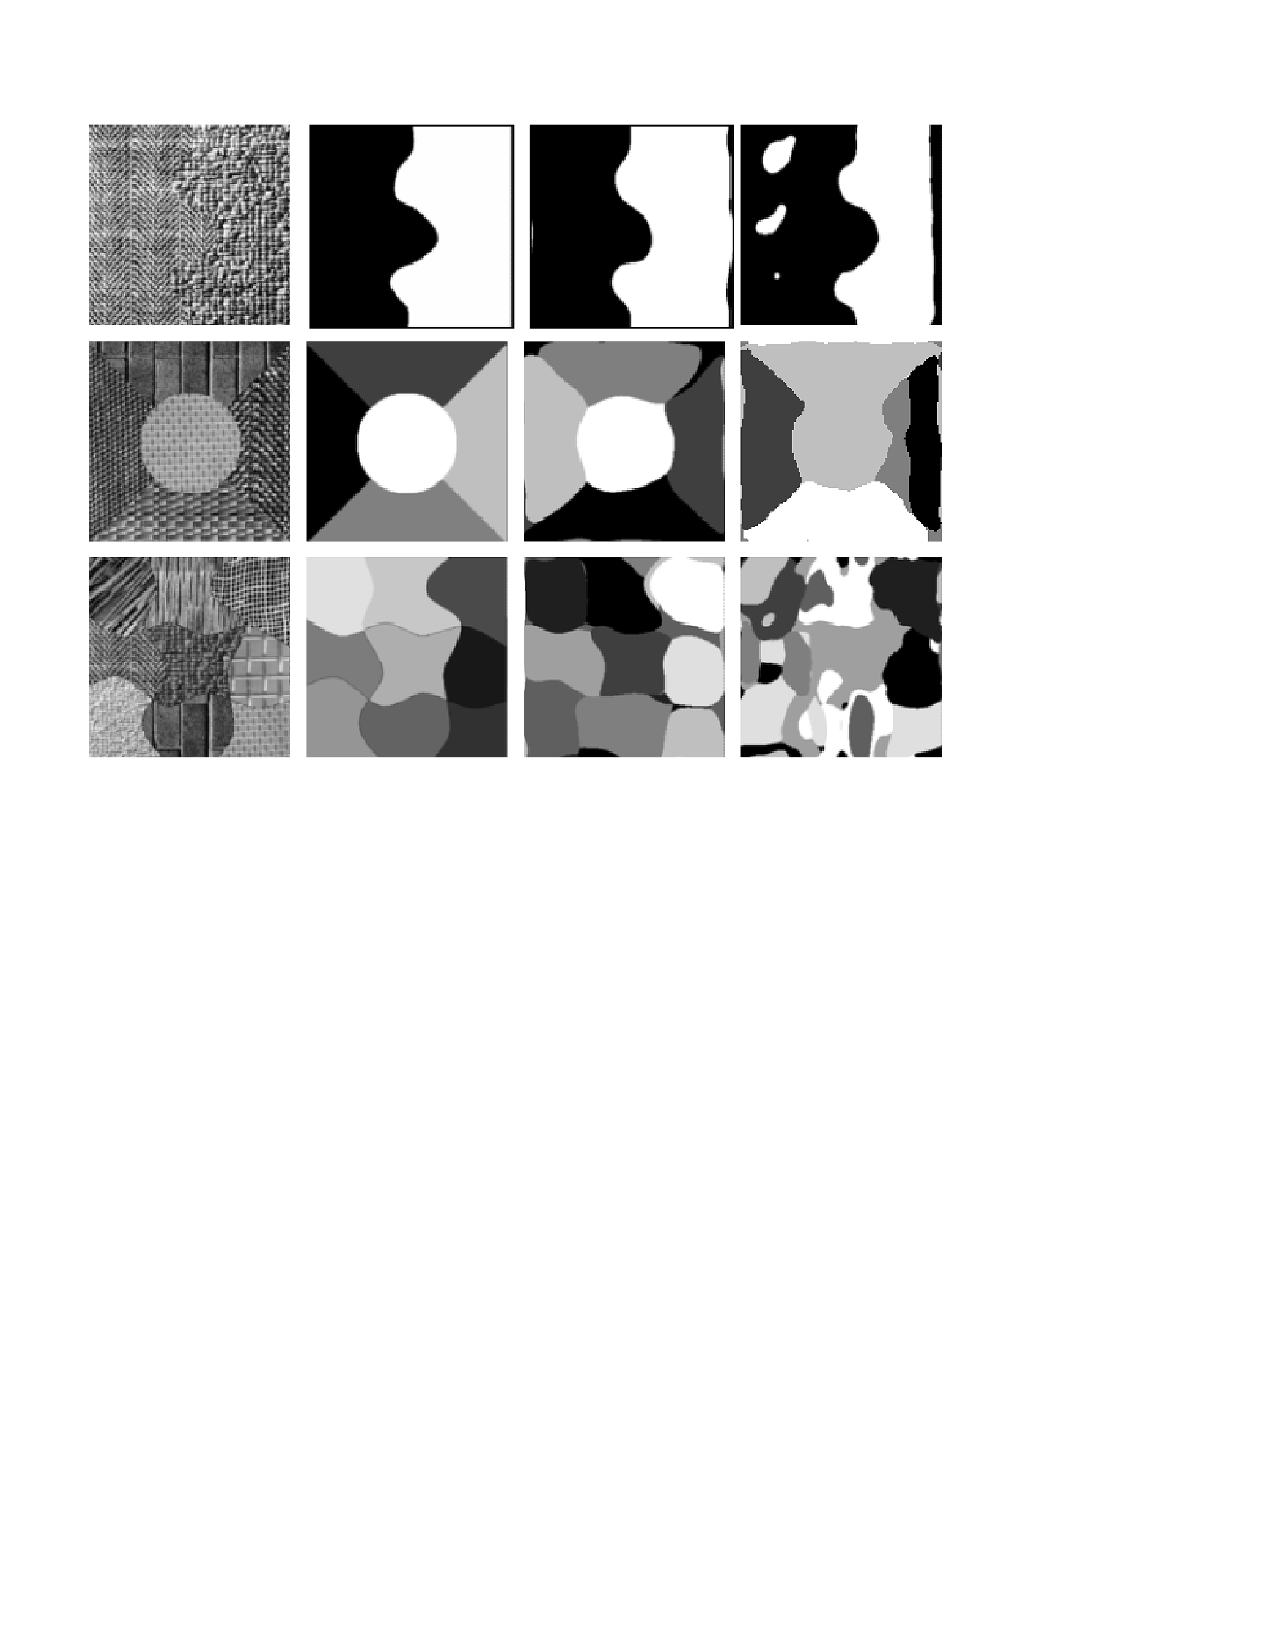
\includegraphics[scale=0.59]{Gabor13}
\caption{Results of segmentation experiments using the $K$-means clustering algorithm.}
\end{figure}
\end{frame}

\section{References}
\subsection{}
\begin{frame}[allowframebreaks]{References}
\linespread{1}

\printbibliography[heading=none]
\end{frame}
{
\nocite{Daugman1985}\nocite{Petkov1995}\nocite{Petkov1997}\nocite{Kruizinga1999}\nocite{Grigorescu2002}\nocite{Petkov2003}\nocite{Grigorescu2003}\nocite{Jain1991}
\setbeamertemplate{logo}{}
\makeatletter
\setbeamertemplate{footline}{
        \leavevmode%
  
  % First line.
  \hbox{%
  \begin{beamercolorbox}[wd=.2\paperwidth,ht=\beamer@decolines@lineup,dp=0pt]{}%
  \end{beamercolorbox}%
  \begin{beamercolorbox}[wd=.8\paperwidth,ht=\beamer@decolines@lineup,dp=0pt]{lineup}%
  \end{beamercolorbox}%
  } %
  % Second line.
  \hbox{%
  \begin{beamercolorbox}[wd=\paperwidth,ht=\beamer@decolines@linemid,dp=0pt]{linemid}%
  \end{beamercolorbox}%
  } %
  % Third line.
  \hbox{%
  \begin{beamercolorbox}[wd=.1\paperwidth,ht=\beamer@decolines@linebottom,dp=0pt]{}%
  \end{beamercolorbox}%
  \begin{beamercolorbox}[wd=.9\paperwidth,ht=\beamer@decolines@linebottom,dp=0pt]{linebottom}%
  \end{beamercolorbox}%
  }%
        }
\makeatother

\begin{frame}
\centering

\includegraphics[width=0.4\paperwidth]{queries.jpg}\\

\includegraphics[width=0.5\paperwidth]{thank_you.png}
\end{frame}
}

